\documentclass[a4paper,11pt]{article}
\usepackage[T1]{fontenc}
\usepackage[utf8]{inputenc}
\usepackage[slovene]{babel}
\usepackage[margin=2.25cm]{geometry}
\usepackage{amsmath,graphicx,booktabs,siunitx}
\sisetup{output-decimal-marker={,},group-separator={\,},group-minimum-digits=4}
\setlength{\parindent}{0pt}
\setlength{\parskip}{4pt}
\raggedbottom
\begin{document}

{\small Univerza v Ljubljani, Fakulteta za strojništvo \hfill Napredna računalniška orodja}\par
\smallskip
{\centering
{\LARGE\bfseries Izračun porazdelitve temperature\\ v prerezu hlajene turbinske lopatice\par}
{\large Poročilo prve faze: priprava in preverjanje sistema enačb}\par
\smallskip
{\normalsize \textbf{Jaka Jaki}\quad Vpisna številka 23241186}\par
}

\section{Uvod in opis problema}
V lopatici plinske turbine toplota prehaja iz vročega plina skozi kovinsko steno do zraka v hladilnih kanalih. Ker se debelina stene in razdalja do najbližjega kanala vzdolž prereza spreminjata, pričakujemo razlike v temperaturi materiala. Zanima nas, kakšno temperaturno polje se vzpostavi pri stacionarnem obratovanju in kolikšna je najvišja temperatura lopatice.

Namen prve faze je na podlagi podane mreže in robnih pogojev sestaviti sistem enačb za temperature v vozliščih. Sistem smo v MATLAB-u preverili na referenčnem primeru, izračunali temperaturno polje za tri gostote mreže lopatice in pripravili binarne datoteke za nadaljnje izračune.

\section{Fizikalni model in vhodni podatki}
Prerez z osmimi hladilnimi kanali prikazuje slika~\ref{fig:prerez}. Obravnavamo dvodimenzionalno stacionarno prevajanje brez notranjih virov toplote. Za nikljevo superzlitino privzamemo konstantno toplotno prevodnost \(k=\SI{22}{\watt\per\metre\per\kelvin}\). Temperatura v materialu zato zadošča Laplaceovi enačbi \(\nabla^2 T=0\).

\begin{figure}[ht]
\centering
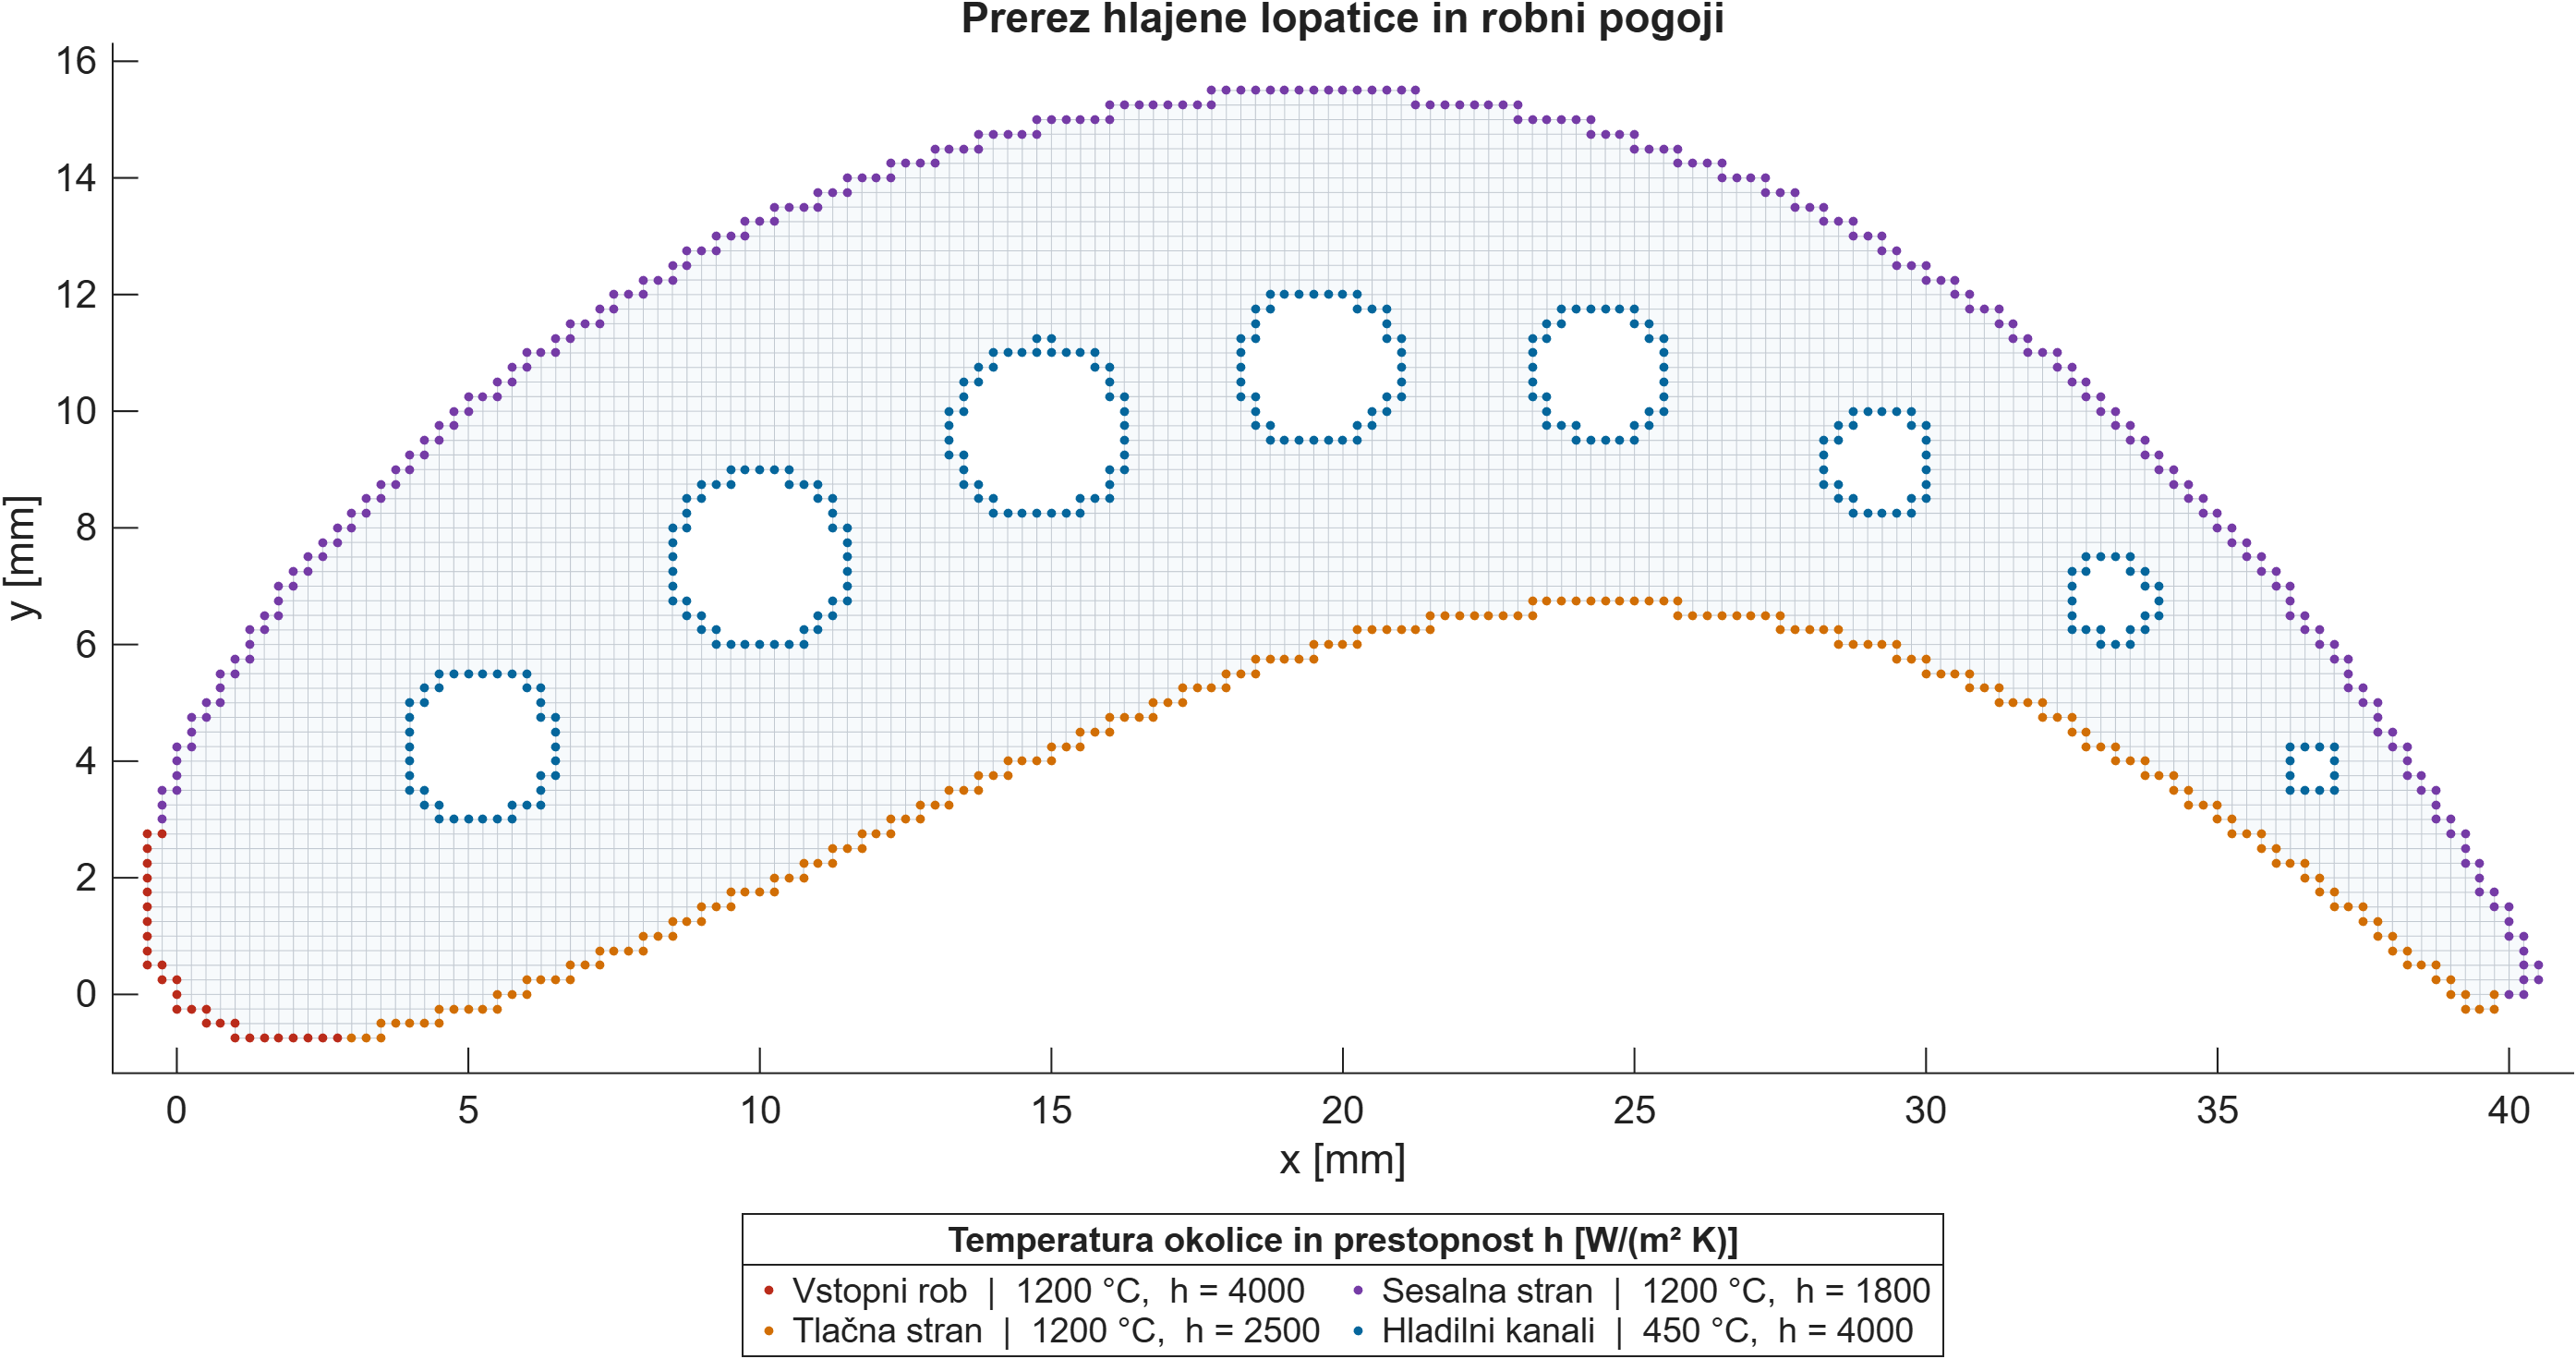
\includegraphics[width=.85\linewidth]{slike/lopatica.png}
\caption{Osnovna mreža iz \texttt{lopatica\_mreza.txt} z razmikom \(\Delta x=\SI{0.25}{\milli\metre}\). Vsaka barvna točka je vozlišče z robnim pogojem. Modre točke obdajajo hladilne kanale; sive črte so stranice celic v materialu.}
\label{fig:prerez}
\end{figure}

Na zunanjem obodu je temperatura plina povsod \SI{1200}{\degreeCelsius}. Vstopni rob, tlačno in sesalno stran ločimo, ker imajo različne prestopnosti \(h\), po vrsti 4000, 2500 in \SI{1800}{\watt\per\square\metre\per\kelvin}. V vseh kanalih je temperatura zraka \SI{450}{\degreeCelsius}, prestopnost pa \SI{4000}{\watt\per\square\metre\per\kelvin}. Te temperature pripadajo tekočinama. Temperaturo stene izračunamo kot del rešitve.

\subsection{Zapis mreže in robnih pogojev}
Funkcija \texttt{preberiMrezo} prebere tri bloke: vozlišča, celice in robne pogoje. Zapise vozlišč in celic uredi po ID ter preveri, ali je vsak pričakovani ID prisoten natanko enkrat. Koordinate v metrih shrani v matriko \texttt{mesh.xy} velikosti \(N\times2\). Vrstica \(i+1\) vsebuje koordinati vozlišča z vhodnim ID \(i\).

Vsaka od \(M\) vrstic matrike \texttt{mesh.cells} vsebuje štiri indekse tipa \texttt{uint32}, povečane za ena zaradi indeksiranja v MATLAB-u. Oglišča si sledijo od zgornjega levega prek spodnjega levega in spodnjega desnega do zgornjega desnega. Vsak element strukture \texttt{mesh.bc} vsebuje oznako skupine, tip pogoja, predpisano vrednost, prestopnost in seznam vozlišč. Bralnik zazna tudi večkratno dodelitev pogoja istemu vozlišču.


\section{Diskretizacija in sestavljanje sistema enačb}
Z metodo končnih razlik vsakemu vozlišču priredimo eno vrstico sistema \(AT=b\). Koeficiente ob temperaturah zapišemo v ustrezne stolpce matrike \(A\), znani člen na desni strani enačbe pa v \(b_i\).
Funkcija \texttt{najdiSosede} oceni \(\Delta x\) z mediano širin celic in s toleranco \(10^{-6}\Delta x\) preveri položaje oglišč. Iz štirih usmerjenih stranic vsake celice sestavi redko matriko. Prišteje ji njeno transponirano matriko in tako dobi simetrične uteži \(w_{ij}\): vrednost 1 pomeni, da stranica med vozliščema \(i\) in \(j\) pripada eni celici, vrednost 2 pa, da jo delita dve.

Funkcija \texttt{razvrstiVozlisca} prešteje celice ob vozlišču. Ena pomeni zunanji kot, dve sosednji celici raven rob, tri notranji kot in štiri notranjost materiala. Preveri tudi število različnih sosedov in ujemanje tako določenega roba s seznami robnih pogojev. V notranjosti imajo vse štiri stranice utež 2. Funkcija \texttt{sestaviSistem} te uteži prepolovi in sestavi vrstico \(T_L+T_R+T_D+T_U-4T_i=0\).

Na robu ohrani uteži \(w_{ij}\). Njihova vsota \(S_i\) je 2 v zunanjem kotu, 4 na ravnem robu in 6 v notranjem kotu. Za pozitivni toplotni tok \(q\) v telo in za prestop toplote veljata enačbi iz tabele~1 projektnih navodil:
\begin{align}
\sum_j w_{ij}T_j-S_iT_i &= -2q\Delta x/k, \label{eq:tok}\\
\sum_j w_{ij}T_j-(S_i+2\mathrm{Bi})T_i &= -2\mathrm{Bi}\,T_\infty,
&\mathrm{Bi}&=h\Delta x/k. \label{eq:prestop}
\end{align}
Na ravnem robu dobi sosed proti notranjosti koeficient 2, soseda vzdolž roba pa 1. Isti postopek pri zasuku roba postavi dvojni koeficient v ustrezni stolpec. Pri predpisani temperaturi program odstrani prispevke sosedov in zapiše \(T_i=T_{\mathrm{rp}}\). Za mreže lopatice uporabimo notranjo enačbo in pogoj prestopa~\eqref{eq:prestop}. Referenčni primer vključuje tudi predpisano temperaturo, dodatni test pa predpisani tok~\eqref{eq:tok}.

Matriko \(A\) program sestavi s funkcijama \texttt{sparse} in \texttt{spdiags}. V vrstici je največ pet neničelnih elementov. Pri najgostejši mreži bi gosta matrika tipa \texttt{double} zavzela približno \SI{759}{\giga\byte}; dejansko zadošča zapis \num{1533657} neničelnih koeficientov.

\section{Binarni zapis sistema in geometrije}
Datoteka \texttt{*\_sistem.bin} vsebuje polja iz tabele~\ref{tab:csr} zaporedno, brez vmesnih bajtov, v zapisu \textit{little-endian}. MATLAB s klicem \verb|find(A.')| obišče elemente prvotne matrike po vrsticah in znotraj vrstice po naraščajočih stolpcih.
\begin{table}[ht]
\centering\small
\begin{tabular}{@{}llll@{}}
\toprule
Polje & Tip & Dolžina & Vsebina \\ \midrule
\(N,\ \mathrm{nnz}\) & \texttt{uint64} & po 1 & število vrstic in število neničelnih koeficientov\\
\texttt{row\_ptr} & \texttt{uint64} & \(N+1\) & odmiki v elementih; prvi 0, zadnji \(\mathrm{nnz}\)\\
\texttt{col\_idx} & \texttt{uint32} & \(\mathrm{nnz}\) & indeks stolpca od 0\\
\texttt{values} & binary64 & \(\mathrm{nnz}\) & vrednosti \(a_{ij}\) v vrstnem redu stolpčnih indeksov\\
\(b\) & binary64 & \(N\) & desna stran po vrstnem redu vozlišč\\
\bottomrule
\end{tabular}
\caption{Zaporedje polj v formatu CSR. Realne vrednosti so zapisane po IEEE~754.}
\label{tab:csr}
\end{table}

Za vrstico \(i\) v C++ preberemo pare \texttt{col\_idx[p]}, \texttt{values[p]} na polodprtem intervalu \(\texttt{row\_ptr}[i]\le p<\texttt{row\_ptr}[i+1]\). Datoteka \texttt{*\_geom.bin} se začne z \(N,M\) (\texttt{uint64}), sledijo pari \(x_i,y_i\) v metrih (binary64) in po štirje indeksi oglišč na celico (\texttt{uint32}, od 0) v vrstnem redu vhodne mreže.


\section{Preverjanje in rezultati}
\subsection{Referenčni primer s 16 vozlišči}
Datoteka \texttt{primer\_predloga\_projekt.txt} vsebuje 16 vozlišč in 9 celic, \(\Delta x=\SI{1}{\metre}\) in \(k=\SI{1}{\watt\per\metre\per\kelvin}\). Na desnem robu je \(\mathrm{Bi}=1000\). Za vozlišče z ID~7 zato dobimo
\[
T_3+2T_6-2004T_7+T_{11}=-400\,000.
\]
Ta vrstica hkrati preverja izbiro sosedov, dvojno utež proti notranjosti in predznak prestopa. Funkcija \texttt{izvediPreverjanja} primerja celotno matriko in vektor z neodvisnim prepisom enačbe~(9) iz projektnih navodil.

\begin{table}[ht]
\centering
\begin{tabular}{@{}lll@{}}
\toprule
Količina & Merilo & Rezultat v MATLAB-u \\ \midrule
\(A\), \(16\times16\) & natančna enakost koeficientov & 256 od 256 enakih\\
\(b\), \(16\times1\) & natančna enakost vrednosti & 16 od 16 enakih\\
\(T\) iz \verb|A\b| & \(\max_i|T_i-T_{i,\mathrm{ref}}|\) & \SI{4.25521e-5}{\kelvin}\\
\bottomrule
\end{tabular}
\caption{Rezultati referenčnega testa. Temperature iz navodil so zaokrožene na štiri decimalke; uporabljena toleranca je \SI{5.0001e-5}{\kelvin}.}
\label{tab:test}
\end{table}

Dodatni test na isti geometriji spremeni levi rob v pogoj \(q=\SI{3}{\watt\per\square\metre}\). Na levem zgornjem vogalu preveri koeficiente \((-2,1,1)\), na ravnem delu levega roba pa \((1,-4,2,1)\). V obeh vrsticah je pričakovana desna stran \(-6\).

\subsection{Rezultati za prerez lopatice}
Za vse štiri gostote je program preveril dimenzije, diagonalo, število neničelnih elementov in končnost vrednosti. Pri vseh petih vhodih, vključno z zgledom, je po zapisu prebral obe binarni datoteki. Funkcija \texttt{uvoziSistem} je preverila dolžino datoteke, odmike in urejenost stolpcev. Rekonstruirana \(A\) in \(b\), vse koordinate ter povezljivost so se natančno ujemali z izvirniki.

\begin{table}[ht]
\centering
\begin{tabular}{@{}lrrrrr@{}}
\toprule
Mreža & \(\Delta x\) [mm] & \(N\) & \(\mathrm{nnz}(A)\) &
 \(T_{\min}\) [\si{\degreeCelsius}] & \(T_{\max}\) [\si{\degreeCelsius}]\\ \midrule
Osnovna & 0,25 & \num{5152} & \num{24996} & 641,98 & 1127,07\\
r1 & 0,125 & \num{19837} & \num{97629} & 641,05 & 1128,64\\
r2 & 0,0625 & \num{77785} & \num{385785} & 640,70 & 1129,38\\
r3 & 0,03125 & \num{307993} & \num{1533657} & -- & --\\
\bottomrule
\end{tabular}
\caption{Sestavljeni sistemi in ekstremi direktnih rešitev. Pri r3 je bilo prostih 2,30~GiB pomnilnika, prag programa za direktno rešitev pa je bil 2,35~GiB.}
\end{table}


Na osnovni mreži ima zunanji rob povprečno \SI{920.272}{\degreeCelsius}, stene kanalov pa \SI{726.416}{\degreeCelsius}. Smer prenosa potrjuje vsota \(Q'_g=\sum_{i\in g}h_g\Delta x(T_{\infty,g}-T_i)\): skozi zunanje skupine toplota vstopa, kanali pa odvedejo \SI{76.844}{\kilo\watt\per\metre}. Na treh rešenih mrežah je relativno odstopanje bilance \(\lvert\sum_g Q'_g\rvert/\sum_g\lvert Q'_g\rvert\) manjše od \(3\cdot10^{-14}\).

\section{Zaključek}
Referenčni primer je potrdil sestavo matrike in desne strani. Na vseh treh rešenih mrežah najvišja temperatura lopatice preseže \SI{1100}{\degreeCelsius}. Z zgostitvijo osnovne mreže na r2 se izračunani maksimum zviša za \SI{2.31}{\kelvin}. Za najgostejšo mrežo r3 sta pripravljena in preverjena sistem enačb in geometrija, izračun temperatur pa ostaja odprt.

\smallskip
{\footnotesize\textbf{Viri.} M. Brank, J. Kovačič, J. Povh in L. Kos, \emph{Izračun porazdelitve temperature v 2D prerezih}, UL FS, 2026/27, razdelki 2--4. Gradivo laboratorijskih vaj 2--4 pri istem predmetu. Numerični podatki: projektni dnevnik \texttt{04\_rezultati/testi/povzetek.txt}.}
\end{document}
